\section{SVN}
\subsection{Allgemeines  \"uber Subversion (SVN)}
Apache Subversion (kurz: SVN) ist eine Software zur Versionsverwaltung von Dateien und Verzeichnissen. Es ist ein zentrales Verwaltungssystem. SVN ist unter der Apache-Lizenz 2.0 ver\"offentlicht und somit Open-Source. Bei SVN erfolgt die Versionierung \"uber ein zentrales Repository. Bei einer Ver\"anderung einer Datei oder eines Verzeichnisses werden zwischen dem Repository und dem Arbeitsplatz nur die Unterschiede \"ubertragen. Merkmale eines zentralen Verwaltungssystemes:
\begin{itemize}
    \item Es gibt nur eines Server aber mehrere Workingcopies
    \item Versionsnummern werden zentral vergeben
    \item Versionshistorie ist nur auf dem Server gespeichert
    \item erm\"oglicht Zugriffs- und Rechtemanagement
\end{itemize}

\begin{figure}[h!]
\centering

\includegraphics[width=\textwidth]{subversion_logo.png}
\caption{Subversion Logo}
\label{fig:logo}
\end{figure}

\subsection{Geschichtlicher Hintergrund}
SVN entstand im Jahre 2000 im amerikanischen Unternehmen CollabNet.
Im November 2009 entschloss CollabNet, dass das Projekt (SVN) an die Apache Software Foundation geht. Danach wurde das Projekt von Apache zu Apache Subversion unbenannt.

\subsection{Vorteile gegen\"uber CVS}
\begin{description}
\item[Die wichtigsten Vorteile]~\par
   \begin{itemize}
      \item Versionsschema
      \begin{itemize}
         \item CVS kann nur die Versionsgeschichte von einzelnen Dateien speichern. SVN von Dateien und Verzeichnissen
      \end{itemize}
      \item \"Anderungsverfolgung
        \begin{itemize}
         \item CVS muss bei einer \"Anderung immer die gesamte Datei \"ubertragen
      \end{itemize}
      \item Umbenennungen und Verschiebungen
              \begin{itemize}
         \item Bei einer Umbenennung oder Verschiebung einer Datei wird in CVS die gesamte Versionsgeschichte gel\"oscht
      \end{itemize}
      \item L\"oschmarkierung von Verzeichnissen
              \begin{itemize}
         \item In CVS k\"onnen nur leere Verzeichnisse gel\"oscht werden
      \end{itemize}
   \end{itemize}
\end{description}
 
 \subsection{Vorteile gegen\"uber GIT}
\begin{description}
\item[Die wichtigsten Vorteile]~\par
   \begin{itemize}
      \item Kostenfrei
      \item Sehr gut getestet
      \item Sehr aktuell, da es stetig weiterentwickelt wird von Apache
      \item Sehr gute Unterst\"utzung von IDE's und Shared Hosting Anbietern (z.B. SourceForge)
         \item Einfache Handhabung
   \end{itemize}
\end{description}
 
\subsection{Die Architektur von Subversion}
Subversion ist auf einem Client-Server-Modell aufgebaut. Auf dem Computer des Benutzers wird ein Client ausgef\"uhrt. Dieser kann \"uber verschiedene Verbindungsarten auf den Server zugreifen. Die ganzen Information \"uber Dateien (Informationen \"uber Zust\"ande, Versionen, Kommentare) und die Dateien selbst liegen auf dem Server. Das Repository selbst, welches auf dem Server liegt, kann entweder in einer BerkleyDB-Datenbank oder direkt auf dem Dateisystem gespeichert werden. Derzeit gibt es drei Zugriffsvarianten:
\begin{itemize}
    \item HTTP / HTTPS
    \item SVN (subversioneigenes \"Ubertragungsprotokoll)
    \item FILE (lokaler Zugriff)
\end{itemize}
\newpage
\begin{figure}[!htbp]
\centering
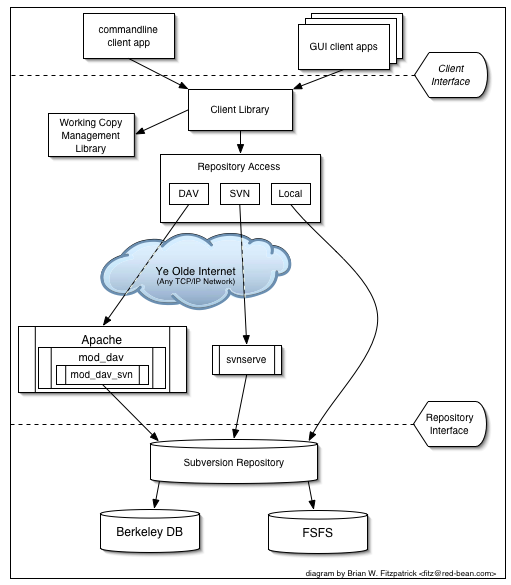
\includegraphics[height=15cm]{subversion_architektur.png}
\caption{Subversion Architektur}
\label{fig:logo}
\end{figure}

\subsection{Die Komponenten von Subversion}
Subversion besteht aus verschiedenen Softwareteilen:
\begin{itemize}
    \item svn
        \begin{itemize}
            \item Kommandozeilenprogramm
        \end{itemize}
    \item svnversion
        \begin{itemize}
            \item Schreibt die Revisionsnummer der Arbeitskopie in die Standartausgabe
        \end{itemize}
    \item svnlook
        \begin{itemize}
            \item Werkzeug um ein Projektarchiv zu untersuchen
        \end{itemize}
    \item svnadmin
        \begin{itemize}
            \item Werkzeug um ein Projektarchiv zu erstellen, zu ver\"andern oder zu reparieren
        \end{itemize}
    \item mod\_dav\_svn
        \begin{itemize}
            \item Plugin f\"ur den Apache-HTTP Server um ein Projektarchiv  \"uber ein Netzwerk verf\"ugbar zu machen
        \end{itemize}
    \item svnserve
        \begin{itemize}
            \item Serverprogramm; Andere M\"oglichkeit um Projektarchiv \"uber ein Netzwerk verf\"ugbar zu machen (SSH)
        \end{itemize}
    \item svnsync
        \begin{itemize}
            \item Tool, um Revisionen eines Projektarchivs in ein anderes Projektarchiv zu \"uberspielen.
        \end{itemize}
\end{itemize}

\subsection{Begriffe in SVN}
\begin{description}
\item[Bei Subversion sind folgende Begriffe wichtig:]~\par
   \begin{itemize}
        \item Revision
        \item Changeset
            \begin{itemize}
        \item Ein Changeset ist eine Zusammenfassung aller \"Anderungen einer Version. Bei einem Changeset gibt es folgende Notations:
        \begin{itemize}
        \item U = Updated
        \item D = Deleted
        \item A = Added
      \end{itemize}
      \end{itemize}
      \item Delta / Diff
              \begin{itemize}
         \item Unter Delta / Diff versteht man die Differenzen zwischen zwei Versionen. In SVN werden immer nur die Unterschieden zwischen zwei Versionen festgehalten.
      \end{itemize}
      \item Merge
              \begin{itemize}
         \item Unter Merge versteht man das Zusammenf\"uhren von verschiedenen \"Anderungen in zwei Versionen einer Datei.
      \end{itemize}
       \item Branch
              \begin{itemize}
         \item Ein Branch ist eine Kopie einer Ursprungsversion.
      \end{itemize}
       \item Tag
              \begin{itemize}
         \item Mit einem Tag kann man die einzelnen Versionen beschriften.
      \end{itemize}
   \end{itemize}
\end{description}
 
 \subsection{Terminal - Befehle f\"ur SVN}
 \begin{description}
\item[Neuen Baum auf den lokalen Rechner kopieren:]~\par
   \begin{itemize}
      \item svn checkout [Pfad] [Lokaler Name]
   \end{itemize}
\item[Lokalen Baum aktualisieren:]~\par
   \begin{itemize}
      \item svn update
   \end{itemize}
\item[Lokale Dateien hinzuf\"ugen und l\"oschen:]~\par
   \begin{itemize}
      \item svn add file...
      \item svn remove file...
   \end{itemize}
   \item[\"Ubersicht \"uber lokale \"Anderungen:]~\par
   \begin{itemize}
      \item svn status
   \end{itemize}
      \item[Lokale \"Anderungen ins Repository \"ubertragen:]~\par
   \begin{itemize}
      \item svn commit -m "Beschreibung der Änderungen"~\par
   \end{itemize}
\end{description}

\subsection{Ist SVN noch aktuell?}
SVN wird durchaus auch heutzutage noch verwendet. Jedoch ist seine gr\"o"ste Konkurrenz GIT, welches mittlerweile weiter verbreitet ist. Es gibt aber einen gro"sen Unterschied zwischen GIT und SVN: GIT ist dezentralisiert und SVN zentralisiert. Deshalb wird SVN auch nicht so schnell verschwinden, da beide Systeme ihr Vor- und Nachteile haben.